\section{问题重述与研究思路}

连续降雨后的山区救援同时面临道路中断、地形起伏及固定通信设施受损。题设提供镇龙乡标准场景，其中一个调度中心面向15个服务区配送80个不可拆货箱。运输机的飞行能力受载荷、装载体积、地形爬升和返航电量限制；执行任务时还须保持与固定网关或空中中继的双向通信。

问题一忽略实体机和共享电池时序，仅研究逐服务区的安全载荷和直接往返组批。问题二引入多点多架次、医疗与首批硬时限、其他物资及时性、8架实体机及共享电池周转。问题三在此基础上要求飞行和交接全过程通信连续，并调度2架中继机及6组能源组件。问题四固定第三问任务和通信关系，将服务区划为两组、三组，核算独立执行所需资源。

四问的核心关系是逐级增加约束：第一问提供航段和组批能力基准，第二问确定物流时间表，第三问修复通信缺口并与运输调度协同，第四问评估共享资源被分割后产生的重复配置。本文始终使用相同的节点编号、坐标系、航段能耗和电池周转规则，避免跨问比较混入计算口径变化。

\begin{table}[H]\centering\normalsize
\caption{四问的核心难点、数学对象与求解方法}\label{tab:question_methods}
\begin{tabular}{cll}\toprule
问题 & 关键数学对象 & 求解与验收方式\\\midrule
一 & 单点安全载荷与不可拆货箱组批 & 单调二分、计数状态动态规划\\
二 & 多点路线、时限与共享机体电池 & 四法路线搜索、CP-SAT排程、逐箱回放\\
三 & 双向通信覆盖与运输中继时窗 & 有限候选协调、连续区间链路证书\\
四 & 不可拆任务组件和独立资源峰值 & 两组、三组穷举与库存缺口核算\\\bottomrule
\end{tabular}\end{table}

图~\ref{fig:roadmap}给出统一物理规则、四问求解及最终逐项核验的衔接顺序。
\begin{figure}[H]\centering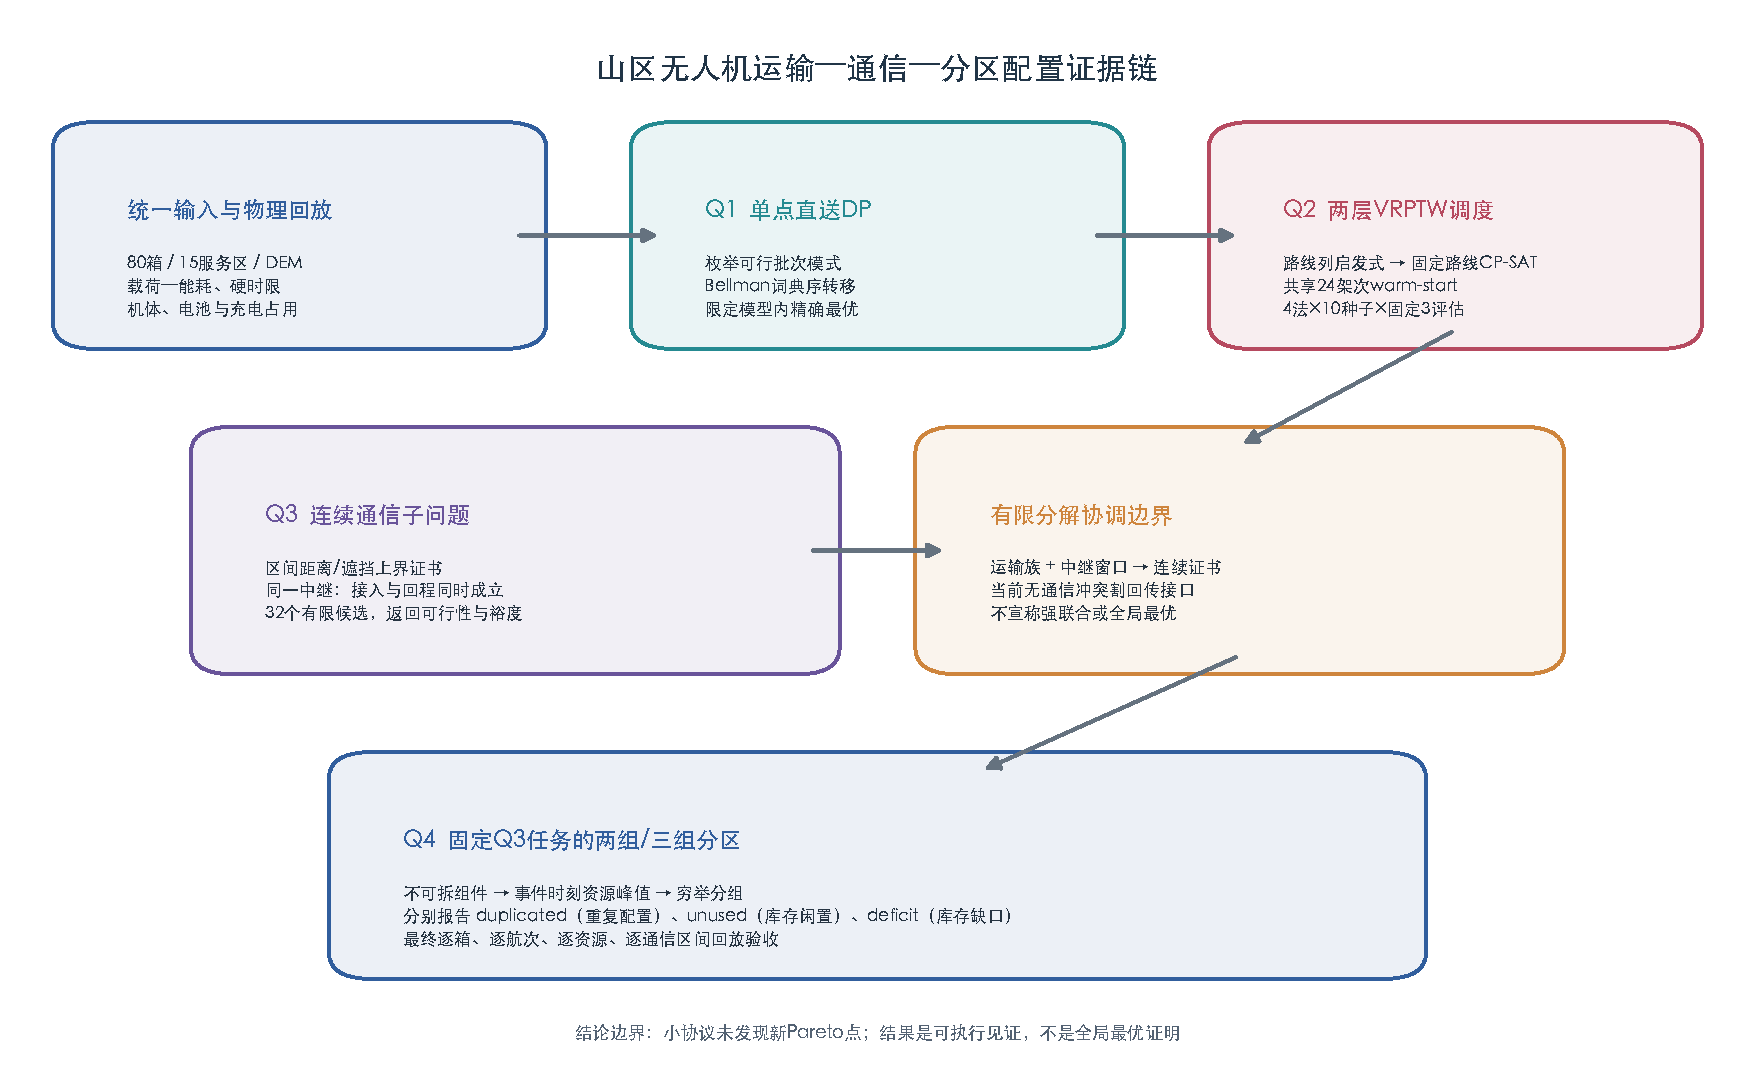
\includegraphics[width=.96\textwidth]{../figures/rigor_pool_20260926/flow_overall_model.pdf}\caption{山区无人机运输、连续通信与分区配置的证据链}\label{fig:roadmap}\end{figure}
